\section{Einleitung}

\begin{frame}
  {Meditieren Sie fünf Minuten!}
  \onslide<+->
  \onslide<+->
  \centering 
  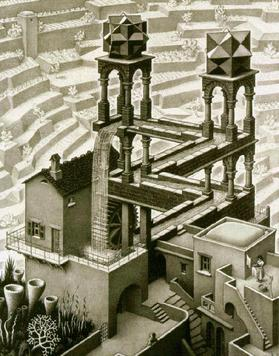
\includegraphics[height=0.7\textheight]{graphics/escher_low}\\
  \grau{\footnotesize M.\,C.\ Escher, \textit{Wasserfall}, Lithografie, 1961.\\
  \url{https://en.wikipedia.org/wiki/File:Escher_Waterfall.jpg}}
\end{frame}

\begin{frame}
  {Das war die Vorbereitung}
  \onslide<+->
  \onslide<+->
  \centering 
  Sie sind jetzt bereit für den schönsten Lexikoneintrag überhaupt!\\
  \Doppelzeile
  \onslide<+->
  \scalebox{1.5}{%
    \begin{avm}
      \[
        phon & \<\> \\
        loc  & \@1 \[ cat|head|dsl & \@1 \]
      \]
    \end{avm}
  }
\end{frame}



\begin{frame}
  {Satzsyntax, und zwar auch noch deutsche!}
  \onslide<+->
  \onslide<+->
  Über Konstituentenstellung müssen wir sowieso noch reden!\\
  \Zeile
  \begin{itemize}[<+->]
    \item Wie lizenziert man die freie Konstituentenstellung im Mittelfeld?
    \item Wie stellt man sicher, dass Köpfe entweder initial oder final in ihrer Phrase stehen?
    \item Wie kommt das Verb in die "`linke Satzklammer"'?
      \Halbzeile
    \item Im Gegensatz zu Stefan finde ich seine Analyse für Verbbewegung\\
      total gut zu verstehen.
    \item \grau{Ich lasse allerdings auch einiges von seiner Argumentation weg.}
  \end{itemize}
  \Zeile
  \onslide<+->
  \centering 
  \grau{\citet[Kapitel~9]{MuellerLehrbuch3}}\\
\end{frame}

\begin{frame}
  {Scrambling}
  \onslide<+->
  \onslide<+->
  Das Verb steht immer \alert{rechts}. Der Rest macht, was er darf.\\
  \onslide<+->
  \Viertelzeile
  \begin{exe}
    \ex[ ]{während Otje [den Artikel] \alert{liest}}
    \ex[ ]{während [den Artikel] Otje \alert{liest}}
    \ex[ ]{während Otje [den Artikel] schnell \alert{liest}}
    \ex[ ]{während Otje schnell [den Artikel] \alert{liest}}
    \ex[ ]{während [den Artikel] Otje schnell \alert{liest}}
    \ex[ ]{während [den Artikel] schnell Otje \alert{liest}}
    \ex[ ]{während schnell Otje [den Artikel] \alert{liest}}
    \ex[ ]{während schnell [den Artikel] Otje \alert{liest}}
    \Viertelzeile
    \onslide<+->
    \ex[*]{während Otje \rot{liest} [den Artikel]}
    \ex[*]{während [den Artikel] \rot{liest} Otje}
    \ex[*]{während \rot{liest} Otje [den Artikel]}
    \ex[*]{während \rot{liest} [den Artikel] Otje}
  \end{exe}
\end{frame}

\begin{frame}
  {Verbbewegung}
  \onslide<+->
  \onslide<+->
  Sie kennen es aus CP\slash IP-Ansätzen. \grau{Darüber ist man sich auch einig.}\\
  \onslide<+->
  \Halbzeile
  \begin{exe}
    \ex[ ]{\gruen{Liest\Sub{1}} [Otje den Artikel \gruen{t\Sub{1}}]?}
    \ex[ ]{\orongsch{Otje\Sub{2}} \gruen{liest\Sub{1}} [\orongsch{t\Sub{2}} den Artikel \gruen{t\Sub{1}}].}
    \ex[ ]{\orongsch{Den Artikel\Sub{2}} \gruen{liest\Sub{1}} [Otje \orongsch{t\Sub{2}} \gruen{t\Sub{1}}].}
    \ex[ ]{\orongsch{Was\Sub{2}} \gruen{glaubst\Sub{1}} [du [dass Otje \orongsch{t\Sub{2}} gelesen hat] \gruen{t\Sub{1}}]?}
  \end{exe}
\end{frame}

\begin{frame}
  {Binäre Strukturen in der VP}
  \onslide<+->
  \onslide<+->
  Das für mich wichtigste Argument für binäre Verzweigung in der VP.\\
  \onslide<+->
  \Halbzeile
  \begin{exe}
    \ex[ ]{während [Otje [morgen [den Artikel [schnell [lesen [müssen wird]]]]]]}
    \Halbzeile
    \ex[ ]{\gruen{Wird} [Otje [morgen [den Artikel [schnell [lesen [müssen \gruen{t\Sub{1}}]]]]]]?}
    \ex[ ]{\orongsch{[Lesen [müssen \gruen{t\Sub{1}}]]} \gruen{wird} [Otje [morgen [den Artikel [schnell \orongsch{t\Sub{2}}]]]].}
    \ex[ ]{\orongsch{[Schnell [lesen [müssen \gruen{t\Sub{1}}]]]} \gruen{wird} [Otje [morgen [den Artikel \orongsch{t\Sub{2}}]]].}
    \ex[ ]{\orongsch{[Den Artikel [schnell [lesen [müssen \gruen{t\Sub{1}}]]]]} \gruen{wird} [Otje [morgen \orongsch{t\Sub{2}}]].}
    \ex[ ]{\orongsch{[Morgen [den Artikel [schnell [lesen [müssen \gruen{t\Sub{1}}]]]]]} \gruen{wird} [Otje \orongsch{t\Sub{2}}].}
  \end{exe}
  \onslide<+->
  \Zeile
  So haben wir jeweils eine \alert{Konstituente}, die ins Vorfeld bewegt werden kann.
\end{frame}

\section{Konstituententellung in HPSG}

\begin{frame}
  {Freie Reihenfolge bei der Komplementation}
  \onslide<+->
  \onslide<+->
  Argumente können in beliebiger Reihenfolge saturiert werden.\\
  \onslide<+->
  \Zeile
  \centering 
  \raisebox{-1.5\baselineskip}{\textit{head-argument-phrase}$\Rightarrow$}%
  \scalebox{0.8}{\begin{avm}
    \[
      loc|cat|subcat & \@1\only<4->{\alert{$\oplus$\@3}} \\
      \alt<3|handout:0>{%
        hd-dtr|loc|cat|subcat & \@1$\oplus$\<\@2\>}{%
          \alert{hd-dtr|loc|cat|subcat} & \alert{\@1$\oplus$\<\@2\>$\oplus$\@3}} \\
      nhd-dtr & \@2 \\
    \]
  \end{avm}}\\
  \onslide<+->
  \onslide<+->
  \Zeile
  \raggedright
  Statt des letzten Arguments irgendeins (\mybox{2}) abbinden:\\
  \Halbzeile
  \begin{itemize}[<+->]\footnotesize
    \item Sowohl \mybox{1} als auch \mybox{3} können leer sein.
    \item Wenn \mybox{1} leer: erstes Argument abbinden
    \item Wenn \mybox{3} leer: letztes Argument abbinden (= alte Version)
    \item Wenn \mybox1 und \mybox3 leer: intransitives Verb
    \item \grau{Der neue Pfad über \textsc{loc} wird unten motiviert.}
  \end{itemize}
\end{frame}

\begin{frame}
  {Mögliche Struktur | Subjekt zuerst abgebunden}
  \onslide<+->
  \onslide<+->
  \centering 
  \scalebox{0.55}{%
    \begin{avm}
      \[ \asort{hd-arg-phr} 
        phon & \phon{den,Artikel,Otje,liest} \\
        loc|cat & \[
          head & \@1 \\
          subcat & \<\> \\
        \] \\
        nhd-dtr & \@3 \[
          phon & \phon{den,Artikel} \\
          loc|cat & \[
            head & \textit{\sl noun} \\
            subcat & \<\> \\
          \]
        \] \\
        hd-dtr & \[ \asort{hd-arg-phr} 
          phon & \phon{Otje,liest} \\
            loc|cat & \[
              head & \@1 \\
              subcat & \<\@3\> \\
            \] \\
            nhd-dtr & \@2 \[ \asort{word} 
              phon & \phon{Otje} \\
              loc|cat & \[
                head & \textit{\sl noun} \\
                subcat & \<\> \\
              \]
            \] \\
            hd-dtr & \[ \asort{word} 
              phon & \phon{liest} \\
              loc|cat & \[
                head & \@1 \\
                subcat & \<\@2 NP\Up{\sl Nom}, \@3 NP\Up{\sl Acc}\> \\
              \]
            \]
        \]
      \]
    \end{avm}
  }
\end{frame}

\begin{frame}
  {Links- und Rechtsköpfigkeit}
  \onslide<+->
  \onslide<+->
  Reihenfolge der Argumentabbindung: nur \alert{Dominanz}\\
  \onslide<+->
  \Viertelzeile
  Abfolge der Konstituenten in Struktur: \alert{Präzedenz}\\
  \grau{\footnotesize Links- und Rechtsköpfigkeit sind nicht modellierbar durch Dominanz!}\\
  \Zeile
  \onslide<+->
  So sollte es sein:\\
  \Halbzeile
  \centering 
  \onslide<+->
  \scalebox{0.8}{%
    \begin{avm}
    \[ \asort{head-arg-phr}
      phon & \alert{\@1 $\oplus$ \@2} \\
      hd-dtr|phon & \@1 \phon{in} \\
      nhd-dtr|phon & \@2 \phon{dem,Buch} \\
    \]
    \end{avm}
  }\onslide<+->\hspace{2em}%
  \scalebox{0.8}{%
    \begin{avm}
    \[ \asort{head-arg-phr} 
      phon & \gruen{\@2 $\oplus$ \@1} \\
      hd-dtr|phon & \@1 \phon{liest} \\
      nhd-dtr|phon & \@2 \phon{das,Buch} \\
    \]
    \end{avm}
  }
\end{frame}

\begin{frame}
  {Übergenerierung}
  \onslide<+->
  \onslide<+->
  Achtung | Wir erlauben bisher \rot{zu viele Strukturen}, nicht zu wenige! \\
  \Zeile
  \centering 
  \onslide<+->
  \scalebox{0.8}{%
    \begin{avm}
    \[ \asort{head-arg-phr}
      phon & \alert{\phon{in,dem,Buch}} \\
      hd-dtr|phon & \@1 \phon{in} \\
      nhd-dtr|phon & \@2 \phon{dem,Buch} \\
    \]
    \end{avm}
  }\onslide<+->\hspace{2em}%
  \scalebox{0.8}{%
    \begin{avm}
    \[ \asort{head-arg-phr}
      phon & \rot{\phon{dem,Buch,in}} \\
      hd-dtr|phon & \@1 \phon{in} \\
      nhd-dtr|phon & \@2 \phon{dem,Buch} \\
    \]
    \end{avm}
  }
\end{frame}

\begin{frame}
  {Linearisierungsregeln | Präzedenz}
  \onslide<+->
  \onslide<+->
  Köpfe wissen selbst, ob sie \alert{initial} oder \alert{final} stehen müssen.\\
  \Zeile
  \onslide<+->
  \centering 
  \begin{minipage}{0.45\textwidth}
    \centering 
    \scalebox{0.7}{
      \begin{avm}
      \[
        phon & \phon{in} \\
        loc|cat & \[
          head & \[ \asort{prep} \alert{initital} & \alert{$+$} \] \\
          subcat & \<NP\Up{\sl Dat}\> \\
        \]
      \]
      \end{avm}
    }\\
    \Zeile

    \onslide<+->
    \Viertelzeile
    \scalebox{0.7}{
      \begin{avm}
      \[
        phon & \phon{hustet} \\
        loc|cat & \[
          head & \[ \asort{verb} \alert{initital} & \alert{$-$} \] \\
          subcat & \<NP\Up{\sl Nom}\> \\
        \]
      \]
      \end{avm}
    }
  \end{minipage}\onslide<+->\hspace{2em}%
  \begin{minipage}{0.45\textwidth}
    Linearisierungsregeln legen fest,\\
    wie \textsc{phon} konkateniert wird.\\
    \Halbzeile
    \begin{itemize}[<+->]
      \item Mit $<$ wird festegelegt,\\
        welches \textsc{phon} zuerst kommt.
        \Halbzeile
      \item Head[\textsc{init\ $+$}]$<$Argument
      \item Argument$<$Head[\textsc{init\ $-$}]
      \Halbzeile
      \item Adjunct[\textsc{pre-mod\ $+$}]$<$Head
      \item Head$<$Adjunct[\textsc{pre-mod\ $-$}]
        \Halbzeile
      \item Specifier$<$Head
    \end{itemize}
  \end{minipage}
\end{frame}


\begin{frame}
  {Verben stehen also unabhängig von der Dominanzfolge VP-final}
  \onslide<+->
  \onslide<+->
  \centering 
  \begin{minipage}{0.45\textwidth}
    \centering 
    \scalebox{0.55}{%
      \begin{avm}
        \[ \asort{hd-arg-phr} 
          phon & \alert{\@6 $\oplus$ \@5 $\oplus$ \@4} \\
          loc|cat & \[
            head & \@1 \\
            subcat & \<\> \\
          \] \\
          nhd-dtr & \@3 \[
            phon & \alert{\@6 \phon{den,Artikel}} \\
            loc|cat & \[
              head & \textit{\sl noun} \\
              subcat & \<\> \\
            \]
          \] \\
          hd-dtr & \[ \asort{hd-arg-phr} 
            phon & \alert{\@5 $\oplus$\ \@4} \\
              loc|cat & \[
                head & \@1 \\
                subcat & \<\@3\> \\
              \] \\
              nhd-dtr & \@2 \[ \asort{word} 
                phon & \alert{\@5 \phon{Otje}} \\
                loc|cat & \[
                  head & \textit{\sl noun} \\
                  subcat & \<\> \\
                \]
              \] \\
              hd-dtr & \[ \asort{word} 
                phon & \alert{\@4 \phon{liest}} \\
                loc|cat & \[
                  head & \@1 \[ \asort{verb} \alert{initial} & \alert{$-$} \]\\
                  subcat & \<\@2 NP\Up{\sl Nom}, \@3 NP\Up{\sl Acc}\> \\
                \]
              \]
          \]
        \]
      \end{avm}
    }
  \end{minipage}\hspace{1em}\onslide<+->%
  \begin{minipage}{0.45\textwidth}
    Ohne Linearisierungsregeln möglich:\\
    \onslide<+->
    \Zeile
    \begin{exe}
      \ex[*]{während liest Otje den Artikel}
      \ex[*]{während liest den Artikel Otje}
      \ex[*]{während Otje liest den Artikel}
      \ex[*]{während den Artikel liest Otje}
    \end{exe}
  \end{minipage}
\end{frame}

\section{Verbbewegung}

\begin{frame}
  {Wiederholung | Bewegungstransformationen}
  \onslide<+->
  \onslide<+->
  \alert{Bewegung} | Erklärt \alert{Abhängigkeiten} zwischen Positionen in Strukturen.\\
  \grau{\footnotesize\textit{Transformationen} sagt man seit der GB-Theorie nicht mehr. Technisch gesehen sind es Transformationen.}\\
  \onslide<+->
  \Zeile
  \centering
  \begin{tabular}{cc}
    \scalebox{0.8}{\begin{forest}
      [CP
        [C$'$
          [C
            [\it dass, rottree]
          ]
          [VP
            [NP
              [\it Matthias, bluetree]
            ]
            [V$'$
              [NP
                [\it Doro]
              ]
              [V
                [\it besucht, gruentree]
              ]
            ]
          ]
        ]
      ]
    \end{forest}} & %
    \visible<4->{\scalebox{0.8}{\begin{forest}
      [CP
        [NP
            [\it Matthias\Sub{2}, bluetree, name=Matthias]
        ]
        [C$'$
          [C
            [\it besucht\Sub{1}, gruentree, name=besucht]
          ]
          [VP
            [t\Sub{2}, bluetree, name=t2]
            [V$'$
              [NP
                [\it Doro]
              ]
              [V
                [t\Sub{1}, gruentree, name=t1]
              ]
            ]
          ]
        ]
      ]
      {\draw [<->, bend left=70, gruen, thick] (t1.south) to (besucht.south);}
      {\draw [<->, bend left=70, trueblue, thick] (t2.south) to (Matthias.south);}
    \end{forest}}} \\
  \end{tabular}
\end{frame}


\begin{frame}
  {Wiederholung | Theorien ohne Transformationen im weiteren Sinn}
  \onslide<+->
  \onslide<+->
  HPSG | \alert{Die gleichen Abhängigkeiten ohne Bewegung}, dafür mit \alert{Strukturteilung}\\
  \grau{\footnotesize Aber nicht unbedingt ohne leere Elemente.}\\
  \onslide<+->
  \Zeile
  \centering 
  \begin{tabular}[h]{cp{0.05\textwidth}c}
    \scalebox{0.6}{\begin{forest}
      [ VP
        [NP
          [\it \alt<1-4|handout:0>{Matthias}{\alert{Matthias\Sub{1}}}]
        ]
        [VP
          [V
            [\it \alt<1-4|handout:0>{besucht}{\gruen{besucht\Sub{2}}}]
          ]
          [VP
            [NP
              [\it Doro]
            ]
            [V
              [\alt<1-4|handout:0>{$\emptyset$}{\alert{t\Sub{1}}}]
              [\alt<1-4|handout:0>{$\emptyset$}{\gruen{t\Sub{2}}}]
            ]
          ]
        ]
      ]
    \end{forest}} && % 
    \onslide<+->\alt<1-4|handout:0>{%
    \scalebox{0.55}{\begin{avm}
      \[ phon & \phon{Matthias, besucht, Doro} \\
        non-hd-dtr & \[ phon & \phon{Matthias} \] \\
        hd-dtr & \[ phon & \phon{besucht, Doro} \\
          hd-dtr & \[ phon & \phon{besucht} \] \\
          non-hd-dtr & \[ phon & \phon{Doro} \\
            non-hd-dtr & \[ phon & \phon{Doro} \] \\
            hd-dtr & \[ phon & \<\> \\
              non-hd-dtr & \[ phon & \<\> \] \\
              hd-dtr & \[ phon & \<\> \]
            \]
          \]
        \]
      \]
    \end{avm}}}{%
    \scalebox{0.55}{\begin{avm}
      \[ phon & \phon{Matthias, besucht, Doro} \\
        non-hd-dtr & \alert{\[ phon & \phon{Matthias } \\ 
          magical-features & \@1
        \]} \\
        hd-dtr & \[ phon & \phon{besucht, Doro} \\
          hd-dtr & \gruen{\[ phon & \phon{besucht} \\
          magical-features & \@2 \]} \\
          non-hd-dtr & \[ phon & \phon{Doro} \\
            non-hd-dtr & \[ phon & \phon{Doro} \] \\
            hd-dtr & \[ phon & \<\> \\
              non-hd-dtr & \alert{\[ phon & \<\> \\
              magical-features & \@1 \]} \\
              hd-dtr & \gruen{\[ phon & \<\> \\
              magical-features & \@2 \]}
            \]
          \]
        \]
      \]
    \end{avm}}%
    }\\
  \end{tabular}  \\
  \Zeile
  \onslide<+->
  \onslide<+->
  \gruen{Heute klären wir für das bewegte Verb, wie die Merkmalsmagie funktioniert.}\\
\end{frame}

\begin{frame}
  {Nicht streng lokale Theorien}
  \onslide<+->
  \onslide<+->
  Auch bei \textit{Bewegung} geht es letztlich darum, wie die magischen Merkmale\\
  in der Struktur einander zugeordnet werden können.\\
  \onslide<+->
  \Zeile
  \begin{minipage}{0.35\textwidth}
    \centering 
    \scalebox{0.8}{\begin{forest}
      [CP
        [NP
            [\it Matthias\Sub{2}, bluetree, name=Matthias]
        ]
        [C$'$
          [C
            [\it besucht\Sub{1}, gruentree, name=besucht]
          ]
          [VP
            [t\Sub{2}, bluetree, name=t2]
            [V$'$
              [NP
                [\it Doro]
              ]
              [V
                [t\Sub{1}, gruentree, name=t1]
              ]
            ]
          ]
        ]
      ]
      {\draw [<->, bend left=70, gruen, thick] (t1.south) to (besucht.south);}
      {\draw [<->, bend left=70, trueblue, thick] (t2.south) to (Matthias.south);}
    \end{forest}}
  \end{minipage}\hspace{1em}\onslide<+->\begin{minipage}{0.6\textwidth}
    Probleme\\
    \Halbzeile
    \begin{itemize}[<+->]\small
      \item Koindizierte bewegte Elemente und Spuren müssen eine Kette (\textit{chain}) bilden.
      \item Dazu muss der Formalismus sie einander zuordnen.
      \item Aus Sicht des bewegten Elements muss \rot{die gesamte c"=Kommando"=Domäne durchsucht werden}.
      \item Der Baum kann beliebig komplex sein, es gibt \rot{kein einfaches Rezept für die Suche} (in der Art von: \textit{aufwärts, dann abwärts: rechts, rechts, links}).
      \item \rot{Bäume} und \rot{Baumdurchsuchungen} machen solche Theorien unnötig komplex und komputational nachteilig.
    \end{itemize}
  \end{minipage}
\end{frame}

\begin{frame}
  {Streng lokale Theorien}
  \onslide<+->
  \onslide<+->
  In einer lokalen Theorie müssen die relevanten Informationen\\
  \alert{am jeweiligen "`Knoten"' verfügbar sein}. Man durchsucht keine Bäume!\\
  \onslide<+->
  \Viertelzeile
  Die Information, dass etwas fehlt, wird an geeigneter Stelle \alert{von Knoten zu Knoten weitergegeben}. Hier steht hinter dem \alert{Doubleslash} jeweils, was fehlt.\\
  \centering 
  \onslide<+->
  \Halbzeile
  \centering
    \scalebox{0.8}{\begin{forest}
        [VP
          [V
            [\it besucht]
          ]
          [VP//V
            [NP
              [\it Matthias]
            ]
            [V$'$//V
              [NP
                [\it Doro]
              ]
              [\gruen<5->{V//V}
              ]
            ]
          ]
        ]
      \end{forest}}\onslide<+->\hspace{3em}\scalebox{0.8}{%
    \gruen{\raisebox{-4.5\baselineskip}{\begin{avm}
      \[
        phon & \<\> \\
        loc  & \@1 \[ cat|head|dsl & \@1 \]
      \]
    \end{avm}
  }}}
\end{frame}

\begin{frame}
  {Ausblick auf die Modellierung}
  \onslide<+->
  Um \alert{Verbbewegung} zu modellieren, brauchen wir keine neuen Regeln, sondern:\\
  \Halbzeile
  \begin{enumerate}[<+->]
    \item Eine Zusammenfassung von \textsc{cat} und \textsc{cont} zu \alert{\textsc{local}} bzw.\ \alert{\textsc{loc}}.
    \Viertelzeile
    \item Eine \alert{lexikalische Verbspur} für alle Verben
      \begin{itemize}[<+->]
        \item Ihr \textsc{phon} ist eine leere Liste.
        \item Ihr Kopfmerkmal \textsc{Doubleslash} bzw.\ \alert{\textsc{dsl} ist strukturgeteilt mit ihrem \textsc{loc}}.
        \item Mit \textsc{dsl} kodiert sie, was fehlt (also das lexikalische Verb selbst).
        \item Sie ist \textsc{initial $-$} wie normale Verben.
        \item Als Kopfmerkmal wird \textsc{loc|cat|head|dsl} in Kopf-Strukturen (VP) weitergegeben.
      \end{itemize}
      \Viertelzeile
    \item Einen Lexikoneintrag per \alert{Lexikonregel für das bewegte Verb}
      \begin{itemize}[<+->]
        \item Sein \textsc{phon} entspricht dem seiner \textsc{lex-dtr} (normales Verb).
        \item Er ist \textsc{initial $+$}, weil er links von der VP steht.
        \item Auf seiner \textsc{subcat} steht eine VP, deren \textsc{loc|cat|head|dsl} \ldots
        \item \ldots\ mit dem \textsc{loc} seiner \textsc{lex-dtr} token-identisch ist.
        \item \gruen{Dadurch wird die gesamte Syntax und Semantik des lexikalischen Verbs\\
          durch die Knoten, deren Kopf die Verbspur ist, in die Verbspur gepumpt.}
        \item \orongsch{Die Verbspur muss daher nicht verbspezifisch sein!}
      \end{itemize}
  \end{enumerate}
\end{frame}

\newcommand{\AvmGa}{%
  \scalebox{0.5}{\begin{avm}
    \[ \asort{word} 
      phon & \<\> \\
      loc & \@1 \[cat|head & \@5 \[dsl & \@1 \]\]
    \]
  \end{avm}}
}

\newcommand{\AvmGb}{%
  \scalebox{0.5}{\begin{avm}
    \@3 \[ \asort{word}
      phon & \phon{hustet} \\
        loc & \@1 \[cat & \[
          head|initial & $-$ \\
          subcat & \<\@2 \[
            loc|cat & \[
              head & \textit{\sl noun} \\
              subcat & \<\> \\
            \]
          \]\>
        \]
      \]
    \]
  \end{avm}}
}

\newcommand{\AvmGc}{%
  \scalebox{0.5}{\begin{avm}
    \[ \asort{v1-lex-rule} 
      phon & \phon{hustet} \\
      loc|cat & \[
        head|initial & $+$ \\
        subcat & \<
          \@4 \[
            loc|cat & \[
              head|dsl & \@1 \\
              subcat & \<\> \\
            \]
          \]
        \>\\
      \]\\
      lex-dtr & \@3 \\
    \]
  \end{avm}}
}

\newcommand{\AvmGd}{%
  \scalebox{0.5}{\begin{avm}
    \@2 \[ \asort{word} 
      phon & \phon{Matthias} \\
    \]
  \end{avm}}
}

\newcommand{\AvmGe}{%
  \scalebox{0.5}{\begin{avm}
    \@4 \[ \asort{hd-arg-phr} 
           phon & \phon{Matthias}$\oplus$\<\> \\
           loc|cat|head & \@5 \[dsl & \@1 \] \\
    \]
  \end{avm}}
}

\newcommand{\AvmGf}{%
  \scalebox{0.5}{\begin{avm}
    \[ \asort{hd-arg-phr}
      phon & \phon{hustet,Matthias}$\oplus$\<\> \\
    \]
  \end{avm}}
}

\begin{frame}
  {Analyse (ausnahmsweise als Baum)}
  \onslide<+->
  \onslide<+->
  \alert{V1-Satz} | \textit{Hustet Matthias?} \\
  \onslide<+->
  \centering
  \begin{forest}
    [\AvmGf
      [\AvmGc
        [\AvmGb]
      ]
      [\AvmGe
        [\AvmGd]
        [\AvmGa]
      ]
    ]
  \end{forest}
\end{frame}


\section{Details der Analyse}

\begin{frame}
  {Neue Merkmalgeometrie für Zeichen}
  \onslide<+->
  \onslide<+->
  \centering 
  \begin{avm}
    \[
      \asort{sign}
      phon & \textit{\sl list of phoneme strings} \\
      \grau{synsem} & \[
        loc & \[
          cat & \[
            head & \textit{\sl head}\\
            subcat & \textit{\sl list of signs} \\
          \] \\
          cont & \textit{\sl cont} \\
        \]\\
        \grau{nonloc} & \grau{\textit{\sl non-local}} \\
      \]
    \]
  \end{avm}\\
  \onslide<+->
  \Zeile
  \alert{\textsc{nonloc}} und \alert{\textsc{synsem}} brauchen wir ab nächster Woche.\\
\end{frame}

\begin{frame}
  {Lexikonregel für Verben in Nicht-Letzt-Stellung}
  \onslide<+->
  \onslide<+->
  Die Regel bildet eine Verb wie \textit{hustet}, das eine VP verlangt, in der es selbst "`fehlt"' (\textsc{dsl}).\\
  \onslide<+->
  \Zeile
  \centering 
  \begin{avm}
    \[ \asort{v1-lex-rule} 
      loc|cat & \[
      head & \[ \asort{verb}
        initial & $+$ \\
      \] \\
      subcat & \<
        \[ loc|cat & \[
          head & \[ \asort{verb} dsl & \gruen{\@1} \] \\
          subcat & \<\> \\
        \]
      \]
      \> \\
    \]\\
      lex-dtr & \[
        loc & \gruen{\@1} \[
        cat|head & \[
          \asort{verb}
          vform & fin \\
          initial & $-$ \\
        \]
      \]
      \]
    \]
  \end{avm}
\end{frame}

\begin{frame}
  {Verbot nicht-stummer Spuren}
  \onslide<+->
  \onslide<+->
  Verhindert ansonsten mögliche Verbdopplung | \textit{\rot{*Hustet Matthias hustet?}}\\
  \onslide<+->
  \Zeile
  \centering 
  \begin{avm}
    \[ hd-dtr & \[ \asort{word} phon & \textit{\sl non-empty-list} \] \]
  \end{avm}\raisebox{-0.75\baselineskip}{$\Rightarrow$%
  \begin{avm}
    \[ loc|cat|head|dsl & \textit{\sl none} \]
  \end{avm}}
\end{frame}




\newcommand{\AvmGSema}{%
  \scalebox{0.44}{\begin{avm}
    \[ \asort{word} 
      phon & \<\> \\
      loc & \@1 \[
        cat|head & \@5 \[dsl & \@1 \] \\
        cont & \@7 \\
    \]
    \]
  \end{avm}}
}

\newcommand{\AvmGSemb}{%
  \scalebox{0.44}{\begin{avm}
    \@3 \[ \asort{word}
      phon & \phon{besucht} \\
        loc & \@1 \[cat & \[
          head|initial & $-$ \\
          subcat & \<\@2 NP\UpSub{\sl Nom}{\@{10}}, \@6 NP\UpSub{\sl Acc}{\@{11}}\>
        \] \\
        cont & \@7 \[ restr & \< \[ \asort{visit-rel} agent & \@{10} \\ other & \@{11} \] \> \] \\
      \]
    \]
  \end{avm}}
}

\newcommand{\AvmGSemc}{%
  \scalebox{0.44}{\begin{avm}
    \[ \asort{v1-lex-rule} 
      phon & \phon{besucht} \\
      loc|cat & \[
        head|initial & $+$ \\
        subcat & \<
          \@4 \[
            loc|cat & \[
              head|dsl & \@1 \\
              subcat & \<\> \\
            \]
          \]
        \>\\
      \]\\
      lex-dtr & \@3 \\
    \]
  \end{avm}}
}

\newcommand{\AvmGSemd}{%
  \scalebox{0.44}{\begin{avm}
    \@2 \[ \asort{word} 
      phon & \phon{Matthias} \\
      loc|cont|ind & \@{10} \\
    \]
  \end{avm}}
}

\newcommand{\AvmGSemdd}{%
  \scalebox{0.44}{\begin{avm}
    \@6 \[ \asort{word} 
      phon & \phon{Doro} \\
      loc|cont|ind & \@{11} \\
    \]
  \end{avm}}
}

\newcommand{\AvmGSeme}{%
  \scalebox{0.44}{\begin{avm}
    \@4 \[ \asort{hd-arg-phr} 
           phon & \phon{Matthias,Doro}$\oplus$\<\> \\
           loc & \[
             cat & \[
               head & \@5 \[dsl & \@1 \] \\
               subcat & \<\> \\
             \] \\
             cont & \@7 \\
           \]\\
    \]
  \end{avm}}
}

\newcommand{\AvmGSemee}{%
  \scalebox{0.44}{\begin{avm}
    \@4 \[ \asort{hd-arg-phr} 
           phon & \phon{Doro}$\oplus$\<\> \\
           loc & \[
             cat & \[
               head & \@5 \[dsl & \@1 \] \\
               subcat & \<\@2\>
             \] \\
             cont & \@7 \\
           \] \\
    \]
  \end{avm}}
}

\newcommand{\AvmGSemf}{%
  \scalebox{0.44}{\begin{avm}
    \[ \asort{hd-arg-phr}
      phon & \phon{besucht,Matthias,Doro}$\oplus$\<\> \\
      cont & \@7 \\
    \]
  \end{avm}}
}

\begin{frame}
  {Die Semantik gibt es umsonst!}
  \onslide<+->
  \onslide<+->
  \centering
  \vspace{-1.75\baselineskip}
  \begin{forest}
    [\AvmGSemf
      [\AvmGSemc
        [\AvmGSemb]
      ]
      [\AvmGSeme
        [\AvmGSemd]
        [\AvmGSemee
          [\AvmGSemdd]
          [\AvmGSema]
        ]
      ]
    ]
  \end{forest}
\end{frame}



\section{Nächste Woche}

\begin{frame}
  {Vorbereitung}
  \onslide<+->
  \onslide<+->
  \centering 
  \large
  Nächste Woche reden wir über Fernabhängigkeiten wie Vorfeldbesetzung.\\
  \onslide<+->
  \Zeile
  \rot{Sie sollten dringend vorher aus dem HPSG-Buch\\
  von Kapitel 10 die Seiten 163--171 lesen!}\\
  \onslide<+->
  \Viertelzeile
  Das sind \gruen{9} Seiten.\\
\end{frame}
